% Created 2016-12-17 Sat 16:57
\documentclass[10pt,conference,compsocconf]{IEEEtran}
\usepackage[utf8]{inputenc}
\usepackage[T1]{fontenc}
\usepackage{fixltx2e}
\usepackage{graphicx}
\usepackage{grffile}
\usepackage{longtable}
\usepackage{wrapfig}
\usepackage{rotating}
\usepackage[normalem]{ulem}
\usepackage{amsmath}
\usepackage{amssymb}
\usepackage{textcomp}
\usepackage{amssymb}
\usepackage{capt-of}
\usepackage{hyperref}
\usepackage{bm}
\usepackage{svg}
\usepackage{graphicx}
\graphicspath{{pics/}}
\usepackage[margin=1in]{geometry}
\usepackage{subfig}
\graphicspath{{pics/}}

\def\arraystretch{1.7}
\author{Laurent Lejeune, Tatiana Fountoukidou, Guillaume de Montauzon}
\date{\today}
\title{Group 97: Road Segmentation}
\hypersetup{
	pdfauthor={Laurent Lejeune, Tatiana Fountoukidou, Guillaume de Montauzon},
	pdftitle={Group 97: Road Segmentation},
	pdfkeywords={},
	pdfsubject={},
	pdfcreator={Emacs 25.1.1 (Org mode 8.3.6)}, 
	pdflang={English}}
\begin{document}
	
\maketitle
	
\section{Introduction}
  The goal of this project is to classify roads in satellite images. An example
  image to segment is shown on figure~\ref{fig:example}.
  We start from a baseline where basic features are extracted and classified. We then describe a more elaborate attempt using a feature set made of Scale Invariant Feature Transform (SIFT) and Hough line transform among others. Generic classifiers similar to our baselines are applied and their predictions are refined using a structured output model called
  structured SVM. A third attempt makes use of a Convolutional Neural Network.
	\begin{figure}[h]
		\centering
		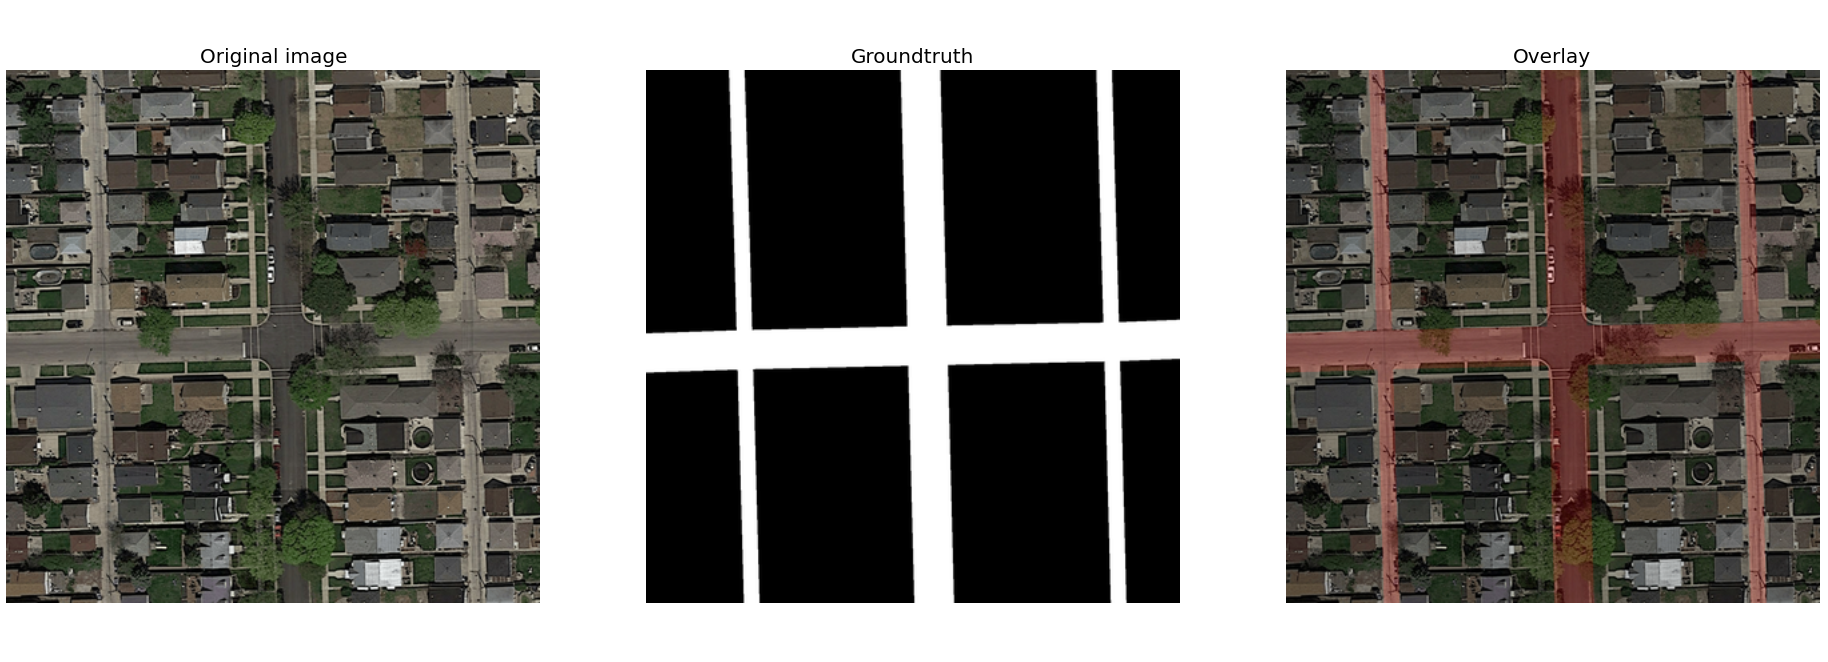
\includegraphics[width=0.45\textwidth]{example.png}
		\caption{Example of training image with its ground-truth}
		\label{fig:example}
	\end{figure}
	
\section{Data exploration}
	The provided training set contains 100 images of size 400x400 along with their
  ground-truth. A total of 6 images are discarded because they either show too few positive class pixels, or some misleading regions such as rail-tracks. 
	We notice that most images are made of grid-like roads, sometimes occluded by trees. 

\section{Baselines}
\subsection{Comparison of classifiers}
\label{baseline_selection}
The images are first cropped into non-overlapping square patches of size $d = 16$. As features,
the mean and variance RGB values are extracted for each patch. As for the
generation of ground-truth samples, a patch $p_i \in \left\{0;1\right\}^{d
  \times d}$ is considered a positive sample if $\frac{\sum_{j}{p_i}}{d^2} >
0.25$, and negative otherwise. A grid search was performed on the
hyper-parameters of three different classifiers: Logistic regression, SVM with
RBF kernel, and random forest. To evaluate the performance, a 5-fold cross
validation is run over the training dataset, and the F-score on the testing set
is calculated for each fold. The mean and the variance of the F-score over the 5
folds is then calculated. The scores for the optimal values of hyper-parameters
are shown in table \ref{table:baselines}. Let us note that random forest is significantly faster to train than SVM. This drives our choice to discard the latter for the remaining of this work.
		\begin{table}[h]
		\centering
		\begin{tabular}{p{0.3\textwidth} c}		
			\textbf{Classifier} &  \textbf{$F-score (\text{mean}\pm \text{std})$}\\
			\hline \hline
			Logistic regression ($\lambda = 1e-2$) & $0.44 \pm 0.02$ \\ \hline
			SVM (rbf kernel, $\lambda = 1e5$) & $0.5 \pm 0.02$ \\ \hline
			\textbf{RF (50 trees, max depth = 10)} & $\bf{0.5 \pm 0.02}$ \\
			\hline
		\end{tabular}
		\caption{\label{table:baselines}Baselines}
		\end{table}
	\subsection{Influence of patch size}
	We examined the impact of the patch size on the classification performance.
	The mean and the variance of the pixels was again used as a feature, and the
	classifier was the baseline RF described above. The F-scores for the different patch sizes are
	shown in table \ref{patch_size}.
	\begin{table}[h]	
	\centering
	\begin{tabular}{p{0.08\textwidth} cccc}
		\hline \hline		
		\textbf{Patch Size} &  8 & 16 & 25 & 32 \\
		\textbf{F-score} &  $0.45 \pm 0.03$ & $0.5 \pm 0.03$ & $0.54 \pm 0.04$ & $0.55 \pm 0.06$ \\
		\hline
	\end{tabular}
	\caption{\label{patch_size}Patch size comparison}
	\end{table}
	Even though the larger the patch size, the better the F-score, we observed that many roads were too narrow to be represented by a larger patch size. The higher score in this case is misleading, since it is calculated on a patch level, and not on a pixel level. Larger patches are more likely to have more than $25\%$ road pixels, but this does not mean that they fully represent a simple road block. This way, although more patches are classified correctly, the overall segmentation mask that comes up is not representative enough. For this reason, the patch size of 16 was kept, as more appropriate to capture the different road widths. For the rest of the work, the performance of the random forest (RF) classifier for patches of size 16 will be used as the baseline.
\section{Structured SVM approach}
  Prior to feature extraction, our images are pre-segmented using	SLIC
  Superpixels (Simple Linear Iterative Clustering) \cite{achanta12}, which
  groups pixels in mid-level regions in an iterative manner. The algorithm
  starts from a regular grid of cluster centers and iteratively updates the
  labels of their neighboring centers based on a distance measure. Compared to square patches, superpixels allow to extract more discriminative regions.
  The next section describes the feature extraction and their encoding.
\subsection{Feature extraction}
\begin{figure}[htb]
\centering
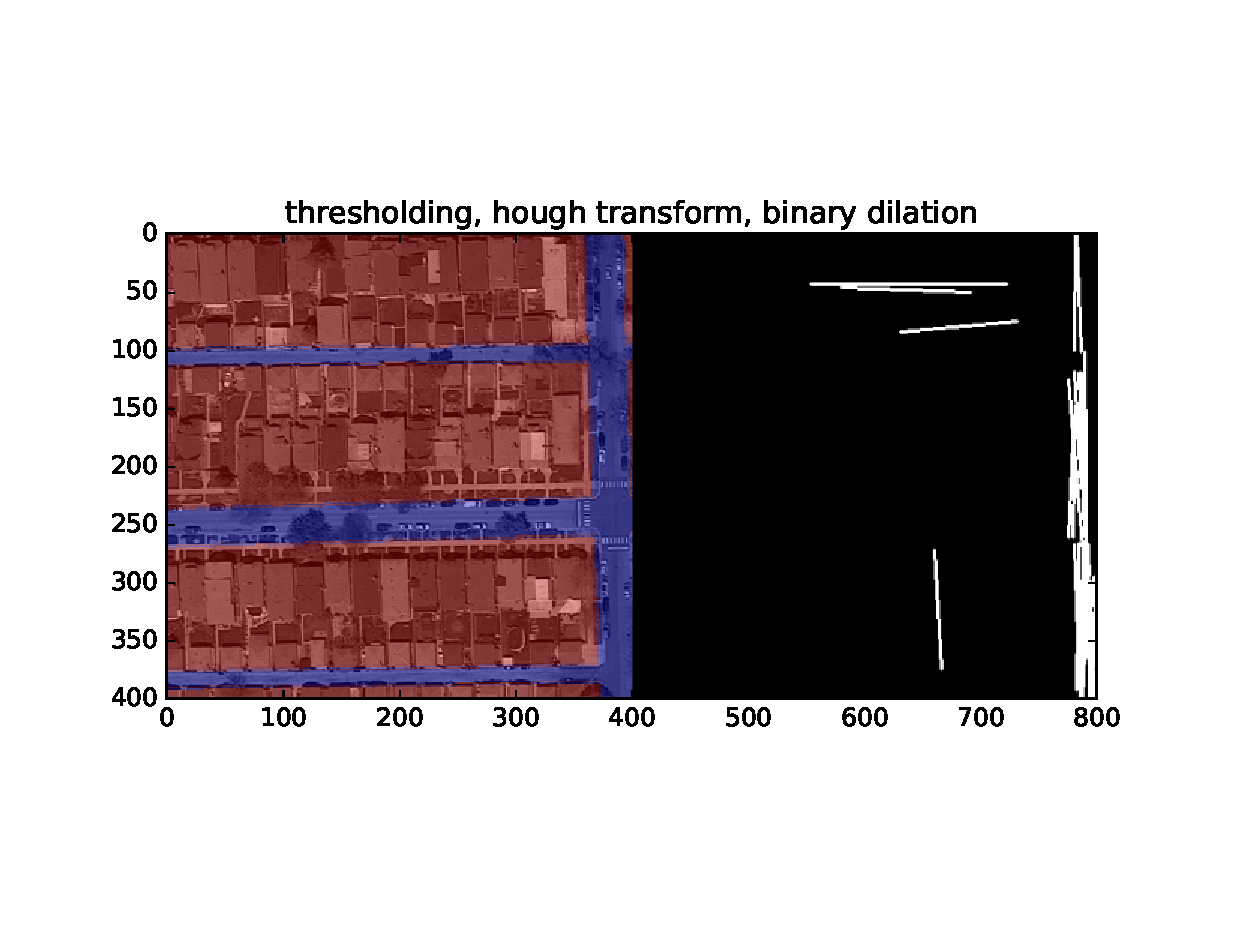
\includegraphics[width=0.35\textwidth]{ex_hough.eps}
\caption{\label{fig:hough}
Example of a hough transform. Left: Input image with the ground-truth overlay. Right: 20 lines with lowest color variance.}
\end{figure}

Following an exploration of the related literature~\cite{fulkerson09}, we select a set of features to extract.
\begin{itemize}
\item\emph{SIFT (Scale-Invariant Feature Transform) \cite{lowe04}}: This descriptor is used extensively in computer-vision applications. It computes a histogram of oriented gradients on $16 \times 16$ windows centered at a keypoint and gives a descriptor of 128 scalar values. The keypoint detection step is not performed, instead we extract the descriptors on a dense grid at canonical scale and orientation. As we require that each segment be represented by a single feature vector, we encode the dense SIFT descriptors contained in a given segment in a "bag-of-features" manner through the following steps: 
\begin{enumerate}
\item Based on a sufficiently large number of SIFT descriptors computed on 10 images, we start by fitting a PCA model. We have checked that the explained variance at 60 components is above 99\%.
\item A codebook is generated on the aforementioned training samples. 
\item We then compute a normalized histogram of codes (bag-of-features) in each segment. This gives us a single texture feature vector for mid-level regions.
\end{enumerate}
\item \emph{Hough line transform.} This transformation has already been used in a state-of-the-art method \cite{2016ISPAr41B3..891L}. First, the edge map is computed using a canny edge detector\cite{canny1986computational}. Given some parameters, a set of lines are extracted on the edge maps and sorted based on their RGB variance, i.e. we want to keep the lines along which the color variations is minimal. An example is shown on figure \ref{fig:hough}. As feature, we take the mean value of the hough map on the segment.
\item \emph{Euclidean distance transform.} This straightforward transform is used to compute, at each pixel location, the shortest taxicab distance to an edge pixel. Using as input the canny edge map, we expect this feature to discriminate cluttered regions such as those containing blocks of buildings where the Euclidean distance tends to be smaller. The mean value over the segment is used.
\item \emph{Mean RGB value.} Roads tend to have greyish colors.
\end{itemize}
To summarize, our feature extraction procedure provides a total of 65 features
per superpixel.

\subsection{Refinement of generic models using structured SVM}
\begin{figure}[htb]
\centering
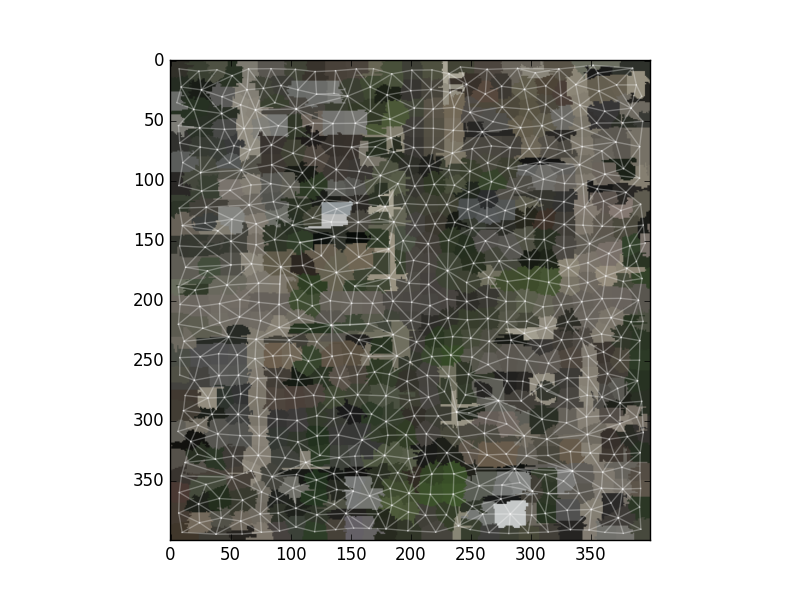
\includegraphics[width=0.23\textwidth]{ex_graph.png}
\caption{\label{fig:graph}
Example of a superpixel-segmented image with connecting edges.}
\end{figure}
   Using structured models \cite{tsochantaridis05}, one can leverage the spatial
   relations between mid-level regions. As shown on figure \ref{fig:graph}, a
   segment considered as road gives a strong prior on the "roadness" of its
   neighboring segment. This is formalized as an undirected graph on which the
   node features are assigned unary potentials. In our case, the unary
   potentials are given by probability estimates given by any generic models such as logistic regression or random forest.
Inspired by \cite{fulkerson09}, the edge costs are made off of two features: The difference in mean LUV color, and the number of pixels that separate two segments (length of separating path). This last feature allows to penalize segments that are "weakly" connected. Indeed, we have verified visually that roads tend to be composed of regular chains of square-like segments, thereby justifying that choice.

Formally, structured models aim at maximizing an energy functions of the form:

 \begin{equation}
 \begin{split}
E_w(X,Y) &= \sum_{i \in \mathcal{V}} E_{data}(y_i;x_i) + \sum_{i,j \in \mathcal{E}} E_{smooth}(y_i;y_j) \\
 &= \mathbf{w}^T \psi(X,Y)
 \end{split}
 \end{equation}

Where \(\mathcal{V}\) is the set of vertices representing a segment and \(\mathcal{E}\) are the edges. The data and smoothness term are combined in the joint-features vector \(\psi\). The variable \(y\) represents the structured labels. The groundtruth labels are extracted analogously to the patch case, meaning a superpixel is labeled as road if more than $25\%$ of its pixels belong to a road. In our setup, any probabilistic regression model (logistic regression, random forest, e.t.c.) can be used for the data term. Following \cite{fulkerson09}, the pair-wise edges potentials are given by:

 \begin{equation}
\phi(c_i,c_j|s_i,s_j) = \frac{L(s_i,s_j)}{1+\lVert s_i - s_j \rVert}
 \end{equation}
Where \(c\) and \(s\) are the mean LUV-space colors. The function \(L\) expresses the length of the shared boundaries between two segments.
The provided code relies on the pyStruct package \cite{muller14}, which implements the cutting-plane algorithm proposed by Tsochantaridis et al \cite{tsochantaridis05}.
\section{Classification}
	Two methods were implemented. The first consists of feature extraction and classification, with the features mentioned aboved. The second consists of training a convolutional neural network (CNN) that takes as input the image and outputs a segmentation mask. Both approaches are described below. 	
	
	\subsection{Classification based on feature vectors}
	The features described above were used to train a random forest ensemble classifier. A grid search to define the hyperparameters of the classifier was performed, and a forest of $50$ trees with maximum depth of $10$ was chosen.
	The CRF refinement step was then performed, and further improved the classification result.
	\subsection{U-net}
	A convolutional neural network designed for image segmentation was used, as
  described in \cite{unet}. U-net is a fully convolutional neural network,
  meaning that it consists exclusively on convolutional and pooling layers, and
  not fully connected layers in the end. As a result, the output of the network
  is not a class assignment for the input, but a feature map. In our case the
  output of the network is a segmentation mask for the input image. The
  structure of the network is shown in figure~\ref{fig:unet_arch} \footnote{In our case the input size is $400 \times 400 \times 3$, and the output is of size $400 \times 400 $}. In the first part of the network, the input image is filtered multiple times, and max pooling is performed to reduce the dimensions of the feature maps. In the second part, the representations that are learned in all the different network depths are combined and up-sampled again, so that an image mask of size equal to the input's can be constructed.
		\begin{figure}[!h]
			\centering
			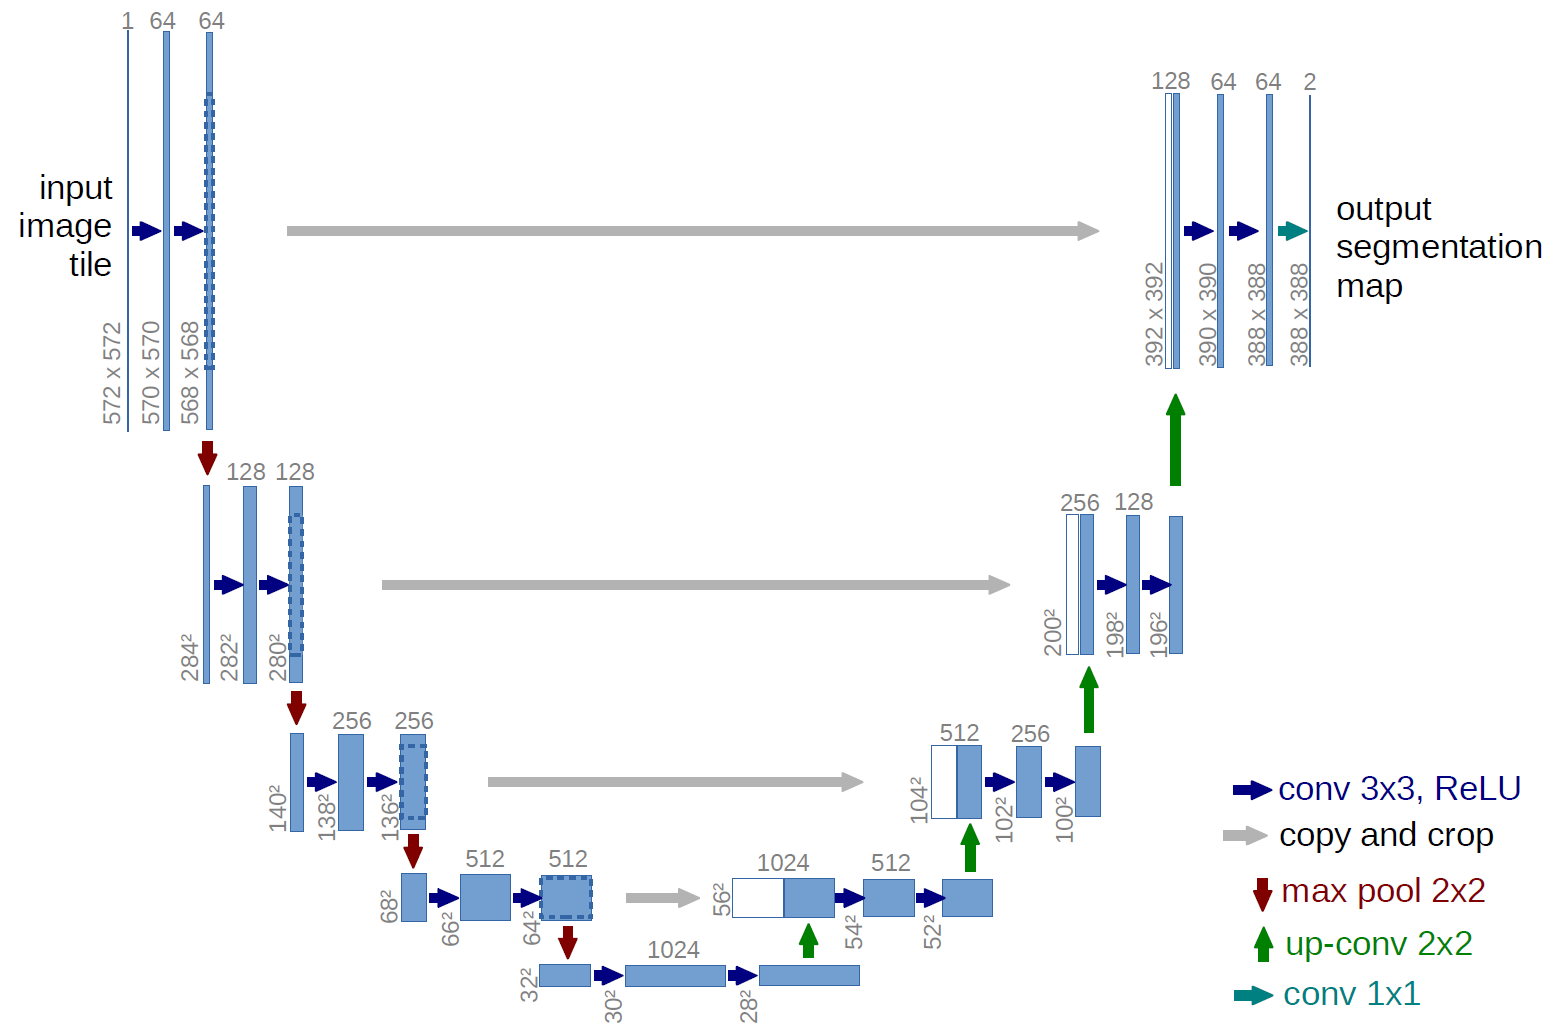
\includegraphics[width=0.45\textwidth]{unet.png}
			\caption{U-net~\cite{unet}}
			\label{fig:unet_arch}
		\end{figure}
\subsubsection{Hyperparameter selection}		
 The network is trained for 100 epochs, but the instance with the lowest validation loss is kept. The loss function is categorical crossentropy, and an Adam optimizer with learning rate of $l=0.0001$ is used. 
 \subsubsection{Data augmentation}
 In order to train such a network (23 convolutional layers), data augmentation is necessary. After dividing our set to training and validation, we therefore augmented the training set, by randomly rotating, flipping, and rescaling the images. 
 An example of some consecutive steps of the network output during training is demonstrated in figure~\ref{steps}.
 
 The experiments for the U-net were run on the keras framework \cite{chollet2015keras}.

 \begin{figure}
\centering
  \captionsetup[subfigure]{labelformat=empty}
  \mbox{\subfloat[]{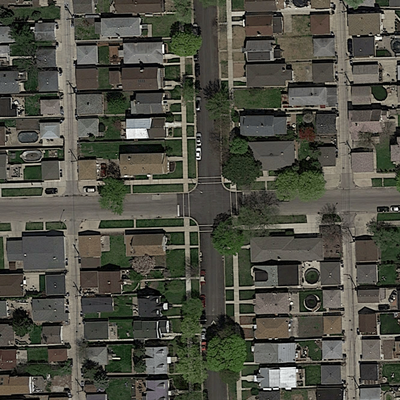
\includegraphics[width=0.3\linewidth]{pics/original.png}}}
  \mbox{\subfloat[]{
\includegraphics[width=0.3\linewidth]{pics/truth.png}}}
  \mbox{\subfloat[]{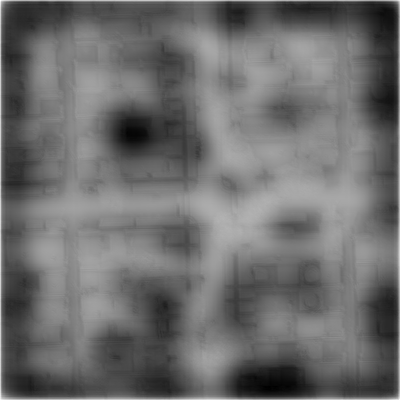
\includegraphics[width=0.3\linewidth]{pics/ep1.png}}}
  \mbox{\subfloat[]{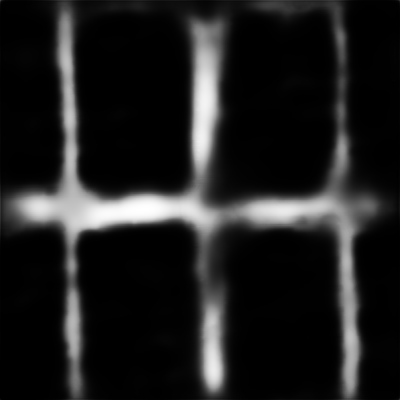
\includegraphics[width=0.3\linewidth]{pics/ep5.png}}}
  \mbox{\subfloat[]{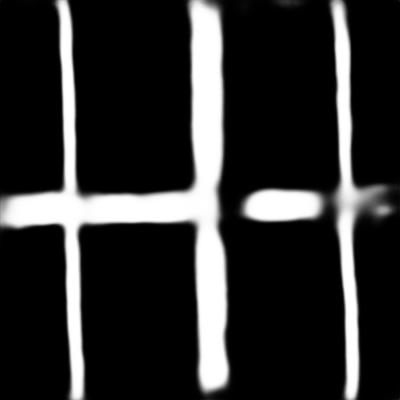
\includegraphics[width=0.3\linewidth]{pics/ep29.png}}}
  \mbox{\subfloat[]{
\includegraphics[width=0.3\linewidth]{pics/ep100.png}}}
\caption{Prediction of unseen image during training using Unet. From left to
right: Image, ground-truth, epoch 1, epoch 5, epoch 30, epoch 100.}\label{steps}
\end{figure}
 
	\section{Results}
	The performance with respect to the regularization parameter for the feature classification case is demonstrated in figure~\ref{fig:reg_ssvm}
		\begin{figure}[!h]
			\centering
			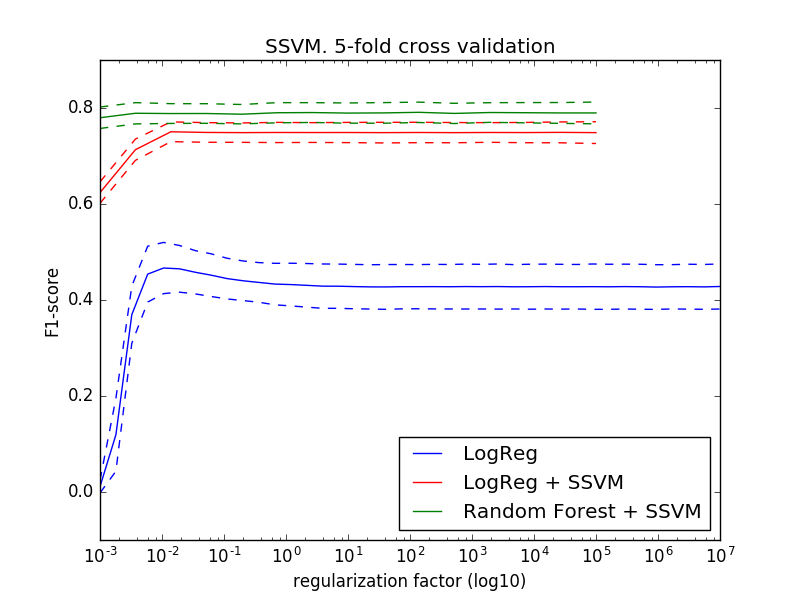
\includegraphics[width=0.4\textwidth]{cross_val_ssvm.png}
			\caption{Comparison of models with and without SSVM.}
			\label{fig:reg_ssvm}
		\end{figure}
The results of a 5-fold cross validation, for the different classification
  approaches that were attempted and described above are shown in table \ref{table:results}  \footnote{Note that for the CNN case only one fold was run due to time contstraints. The reported F-score is on the validation set, and is calculated on a pixel level, contrary to the previous methods that are evaluated on a patch level, and on a superpixel level.}.
		\begin{table}[h]
			\begin{tabular}{p{0.2\textwidth} c}		
				\textbf{Classification method} &  \textbf{$F-score (\text{mean}\pm \text{std})$}\\
				\hline \hline
				Random forest, square patches, basic features [Baseline] & $0.5 \pm 0.02$ \\ \hline
				Logistic regression ($\lambda = 1e-2$), elaborate features& $0.45 \pm 0.02$ \\ \hline
				Random forest (50 trees, max. depth 10), elaborate features& $0.68 \pm 0.03$ \\ \hline
				Random forest, SSVM refinement, elaborate features & $0.79 \pm 0.02$ \\ \hline
				Logistic regression, SSVM refinement, elaborate features& $0.68 \pm 0.02$ \\ \hline
				U-net & $0.9$ \\
				\hline
			\end{tabular}
			\caption{\label{table:results}Overall results}
		\end{table}
	Also, in figure~\ref{example_all} one can see an example image with it's groundtruth, and the predictions of all the different methods.

 \begin{figure}
  \captionsetup[subfigure]{labelformat=empty}
\centering
  \mbox{\subfloat[]{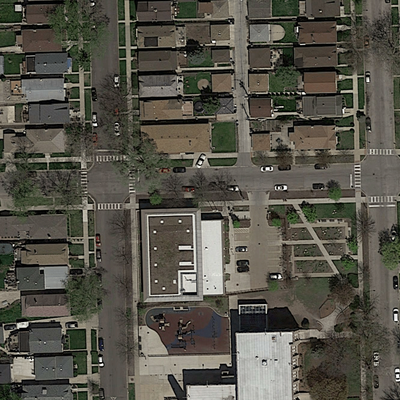
\includegraphics[width=0.3\linewidth]{pics/image2.png}}}
  \mbox{\subfloat[]{
\includegraphics[width=0.3\linewidth]{pics/gt2.png}}}
  \mbox{\subfloat[]{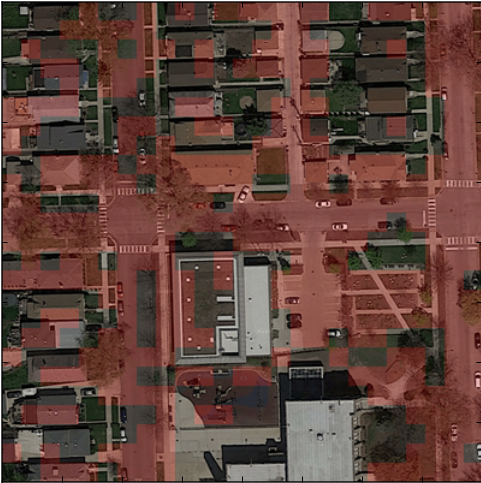
\includegraphics[width=0.3\linewidth]{pics/baseline2.png}}}
  \mbox{\subfloat[]{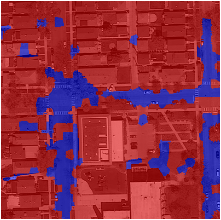
\includegraphics[width=0.3\linewidth]{pics/RF2.png}}}
  \mbox{\subfloat[]{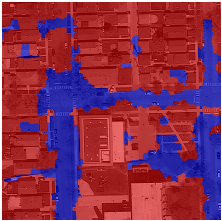
\includegraphics[width=0.3\linewidth]{pics/RFrefined2.png}}}
  \mbox{\subfloat[]{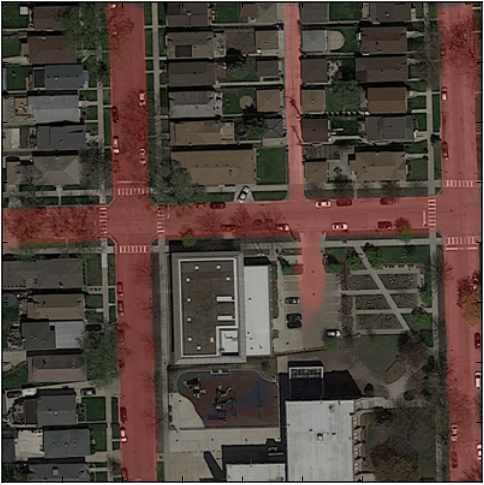
\includegraphics[width=0.3\linewidth]{pics/unet2.png}}}

\caption{Example of predictions on unseen image. From left to right: Image,
  ground-truth, RF with basic features, RF with elaborate features, refined RF, Unet.}\label{example_all}
\end{figure}

\section{Conclusions}
We have described and evaluated three classifiers for segmenting roads in
satellite images. Our results suggest that this application makes great profit
of global information. Indeed, the structured SVM allowed an increase of
10\% in F1-score compared to the patch-by-patch approach. The CNN approach
gives another 11\% increase with respect to SSVM, by effectively learning
appropriate features on top of the data structure.
	\bibliographystyle{ieeetr}
	\bibliography{refs}
\end{document}